\documentclass[11pt]{article}

\usepackage[a4paper,margin=27mm]{geometry}
\usepackage{fontspec}
\usepackage{xeCJK}
\usepackage{unicode-math}
\setmainfont{TeX Gyre Termes}
\setsansfont{TeX Gyre Heros}
\setmonofont{TeX Gyre Cursor}
\setmathfont{TeX Gyre Termes Math}
\setCJKmainfont{Noto Serif CJK SC}
\setCJKsansfont{Noto Sans CJK SC}
\setCJKmonofont{Noto Sans Mono CJK SC}
\usepackage{microtype}
\usepackage{amsthm}
\usepackage{amsmath}
\usepackage{mathtools}
\usepackage{booktabs}
\usepackage{tabularx}
\usepackage{array}
\usepackage{enumitem}
\usepackage{graphicx}
\usepackage{tikz}
\usetikzlibrary{arrows.meta,positioning,fit,calc,backgrounds}
\usepackage{placeins}
\usepackage[numbers,sort&compress]{natbib}
\usepackage{xcolor}
\usepackage{url}
\usepackage{hyperref}
\usepackage[nameinlink,noabbrev]{cleveref}

\hypersetup{
  unicode=true,
  pdftitle={Marked Time Cohomology and Orbitwise Standardization of Indiscrete Arithmetic Action Groupoids},
  pdfauthor={Liang Wang},
  pdfsubject={Marked degree-one cohomology, common-period orbitwise standardization, and the invariant diagonal},
  pdfkeywords={indiscrete action groupoid, marked cocycle, continuous cohomology, orbitwise standardization, arithmetic flow, invariant diagonal},
  colorlinks=true,
  linkcolor=blue!45!black,
  citecolor=green!35!black,
  urlcolor=blue!55!black
}

\setlength{\parindent}{1.35em}
\setlength{\parskip}{0.23em}
\setlength{\emergencystretch}{3em}
\setlist{nosep,leftmargin=2em}
\renewcommand{\arraystretch}{1.16}
\newcolumntype{Y}{>{\raggedright\arraybackslash}X}
\newcolumntype{P}[1]{>{\raggedright\arraybackslash}p{#1}}

\newtheorem{theorem}{Theorem}[section]
\newtheorem{proposition}[theorem]{Proposition}
\newtheorem{lemma}[theorem]{Lemma}
\newtheorem{corollary}[theorem]{Corollary}
\theoremstyle{definition}
\newtheorem{definition}[theorem]{Definition}
\newtheorem{remark}[theorem]{Remark}

\newcommand{\R}{\mathbb R}
\newcommand{\Z}{\mathbb Z}
\newcommand{\Gactual}{G_{\mathrm{actual}}}
\newcommand{\Gstd}{G_{\mathrm{std}}}
\newcommand{\Gammaactual}{\Gamma_p^{\mathrm{actual}}}
\newcommand{\Gammastd}{\Gamma_p^{\mathrm{std}}}
\newcommand{\Qactual}{Q_p^{\mathrm{actual}}}
\newcommand{\Qdisc}{Q_p^{\mathrm{disc}}}
\newcommand{\Ccnv}{C_{\mathrm{cnv}}}
\newcommand{\Zcnv}{Z_{\mathrm{cnv}}}
\newcommand{\Bcnv}{B_{\mathrm{cnv}}}
\newcommand{\Hcnv}{H_{\mathrm{cnv}}}
\newcommand{\cnv}{\mathrm{cnv}}
\newcommand{\Std}{\operatorname{Std}_{\mathrm{coprod}}}
\newcommand{\Indisc}{\operatorname{Indisc}}
\newcommand{\AutR}{\operatorname{Aut}_{\R}}
\newcommand{\Sym}{\operatorname{Sym}}
\newcommand{\Per}{\operatorname{Per}}
\newcommand{\Stab}{\operatorname{Stab}}
\newcommand{\im}{\operatorname{im}}
\newcommand{\id}{\operatorname{id}}
\newcommand{\RouteA}{\textsc{Route A}}
\newcommand{\RouteB}{\textsc{Route B}}
\newcommand{\TupleRejected}{%
  $\begin{gathered}
  (\mathrm{A0\_FAIL},\mathrm{A1\_FAIL},\mathrm{A2\_FAIL},\\
  \mathrm{A3\_FAIL},\mathrm{A4\_FAIL})
  \end{gathered}$}
\newcommand{\TupleActual}{%
  $\begin{gathered}
  (\mathrm{A0\_ANALYTIC\_ARITHMETIC\_ORIGIN},\\
  \mathrm{A1\_WEAK},\mathrm{A2\_FAIL},\mathrm{A3\_FAIL},
  \mathrm{A4\_FAIL})
  \end{gathered}$}
\newcommand{\TupleStandard}{%
  $\begin{gathered}
  (\mathrm{A0\_WEAK\_ARITHMETIC\_RELATION},\\
  \mathrm{A1\_WEAK},\mathrm{A2\_FAIL},\mathrm{A3\_FAIL},
  \mathrm{A4\_FAIL})
  \end{gathered}$}
\newcommand{\TupleUnmarked}{%
  $\begin{gathered}
  (\mathrm{A0\_FAIL},\mathrm{A1\_WEAK},\mathrm{A2\_FAIL},\\
  \mathrm{A3\_FAIL},\mathrm{A4\_FAIL})
  \end{gathered}$}

\title{\textbf{Marked Time Cohomology and Orbitwise Standardization\\of Indiscrete Arithmetic Action Groupoids}}
\author{Liang Wang\\
\small Huazhong University of Science and Technology\\
\small Academic unit and corresponding-author status: AUTHOR TO CONFIRM\\
\small \href{mailto:wangliang.f@gmail.com}{wangliang.f@gmail.com}}
\date{15 August 2026}

\begin{document}
\maketitle

\begin{abstract}
Let a nonempty set carry a right real action and one global indiscrete
topology.  We define a globally continuous, unnormalized nerve cochain
complex and prove, in every finite degree, that cochains with a $T_0$
coefficient target factor through time.  For real coefficients the actual
action groupoid has $H^1_{\mathrm{cnv}}=\R[c]$, $c(x,t)=t$, and its
degree-one coboundaries vanish.  On every unit of the fixed-prime packet,
the source-normalized marked class has isotropy image $(\log p)\Z$.  Strict
maps preserve this subgroup, positive scaled maps transform it covariantly,
and weaker categories admit explicit non-descent.  When all stabilizers are
the same cocompact lattice $H=L\Z$, the same carrier admits a section-free
coproduct of standard $\R/H$ orbit topologies; this construction is fully
faithful with global indiscretization.  Its canonical automorphism extension
has kernel $(\R/H)^Q$, while a split requires choices of orbit origins and is
noncanonical.  The standardized groupoid satisfies
$H^1_{\mathrm{cnv}}=\R^Q$, the full algebraic Cartesian product, and its
coboundaries are generally nonzero.  The continuous identity
$J:G_{\mathrm{std}}\to G_{\mathrm{actual}}$ induces the constant diagonal,
exactly the strict-automorphism invariant subspace.  The packet application
uses only the bare nonempty orbit set: it transfers no count, measure, or
actual quotient topology.  Deterministic finite controls support
reproducibility but replace neither proof nor source verification.  We obtain
no higher standardized cohomology, cohomology topology, trace, determinant,
analytic continuation, or operator lift.

\medskip
\noindent\textbf{Keywords:} marked time cohomology; indiscrete action
groupoid; orbitwise standardization; common period lattice; arithmetic
flow; invariant diagonal
\end{abstract}

\begin{center}
\textbf{中文摘要}
\end{center}
设非空集合带实数右作用及整体不可分拓扑。我们定义整体连续、非正规化的神经上链复形，并证明对每个有限次数，取值于 $T_0$ 群的上链均经时间坐标分解。取实系数时，实际作用群胚满足 $H^1_{\mathrm{cnv}}=\R[c]$，且一次余边界为零。在固定素数包的每个单位上，源归一化标记类的迷向像为 $(\log p)\Z$；严格映射保持它，正比例映射使其协变，而较弱范畴存在明确的不下降反例。若各点稳定子同为余紧格 $H=L\Z$，则同一载体具有不依赖截面的标准 $\R/H$ 轨道拓扑余积，并与整体不可分化构成满且忠实的对应。其典范自同构正合列之核为 $(\R/H)^Q$；选择轨道原点才能得到非典范分裂。标准化群胚满足 $H^1_{\mathrm{cnv}}=\R^Q$，这里是完整代数直积，且标准化一次余边界通常非零。连续恒等函子 $J:G_{\mathrm{std}}\to G_{\mathrm{actual}}$ 诱导常值对角，其像恰为严格自同构不变子空间。固定素数应用只使用非空裸轨道集，不转移计数、测度或实际商拓扑。确定性有限控制仅支持复现，不能替代证明与来源核验。本文不建立更高次标准化上同调、上同调拓扑、迹、行列式、解析延拓或算子提升。

\medskip
\noindent\textbf{中文关键词：} 标记时间上同调；不可分作用群胚；逐轨道标准化；共同周期格；算术流；不变对角

\tableofcontents

\section{Introduction}
\label{sec:introduction}

Periodic time is easy to see set-theoretically and easy to lose
categorically.  If a real action is presented on a Hausdorff circle, its
period lattice is built into the familiar quotient $\R/L\Z$.  If the same
carrier inherits one global indiscrete topology, every continuous map to a
$T_0$ target forgets the unit coordinate.  The marked time cocycle survives,
but the topology no longer separates even distinct orbits.  This paper makes
the comparison without identifying the two topologies.

The arithmetic motivation comes from Deninger's suspension construction.
In arXiv version 4, Section~6 and Theorem~6.1 on physical
pp.~38--39 give the fixed-prime right flow, multiplicative isotropy $p^{\Z}$
at every packet point, and the logarithmic clock; additive time therefore
gives the common stabilizer $(\log p)\Z$ \cite{Deninger2026Dynamical}.
Equations~(38)--(39) there are set parametrizations, not topology transport.
A companion analysis establishes the globally indiscrete topology of the
actual fixed-prime packet \cite{Wang2026PacketSeparation}; another studies
its separated reflections \cite{Wang2026SeparatedReflections}; and a third
supplies the range-first action-groupoid and convolution context
\cite{Wang2026ContinuousConvolution}.  We use those records only at those
ceilings.  The generic theorems below are proved from their stated
hypotheses, so they do not depend on the public availability of a companion.

There are two mathematical layers.  The first is the actual indiscrete
layer.  We compute every finite nerve chart, define the author-specific
complex $\Ccnv^\bullet$, prove $d^2=0$ directly, and show that the full
complex factors through time for $T_0$ coefficients.  In real degree one,
the continuous Cauchy equation leaves precisely the line generated by
$c(x,t)=t$.  Restriction to isotropy then turns the marked class into the
subgroup $\lambda H_x\subset\R$.

The second layer assumes a common cocompact stabilizer $H=L\Z$, $L>0$.
Every orbit receives its standard quotient topology, independently of an
origin, and the carrier receives the coproduct topology.  The ordinary
facts about $\R/H$ and topological coproducts provide background
\cite{EoMTopologicalGroup,EoMHomogeneousSpace,Stacks0B1W}; the same-carrier
construction, its uniqueness, its exact categorical inverse, its
automorphism extension, and its cohomology comparison are proved here.

The central statement is the following comparison, in which $Q=X/\R$ is a
nonempty bare set and $\R^Q$ is the full algebraic Cartesian product.

\begin{theorem}[Main comparison theorem]
\label{thm:main}
Let $X$ be a nonempty globally indiscrete right $\R$-set with
$\Stab_{\R}(x)=H=L\Z$ for every $x$, where $L>0$.  Let $\Gactual$ be its
range-first action groupoid with mark $c(x,t)=t$, and let $\Gstd$ be the
same-set orbitwise standardization.  Then
\begin{equation}
\label{eq:central-map}
\begin{aligned}
 \Hcnv^1(\Gactual;\R)=\R[c]
 &\xrightarrow{\ J^*\ }
 \Hcnv^1(\Gstd;\R)=\R^Q,\\
 \im(J^*)&=(\R^Q)^{\AutR(\Gstd)}\\
 &=\{\text{constant functions }Q\to\R\}.
\end{aligned}
\end{equation}
Here $J:\Gstd\to\Gactual$ is the continuous identity marked functor, and
$\AutR$ means strict time-preserving equivariant automorphisms.  No topology
is imposed on $\R^Q$, either cohomology group, or the automorphism group.
\end{theorem}

This theorem is the paper's center.  The actual collapse is its input, not
its conclusion, and the automorphism computation is a mechanism for the
invariant statement rather than an arithmetic selection principle.  The
proof also keeps the variance straight: $J$ goes from the finer standard
topology to the actual indiscrete topology, while cohomological pullback goes
from actual to standard.

The closest formal action-groupoid lift/descent comparison we found is
Gepner--Meier's Proposition~2.15, printed p.~2647, in compactly generated
weak-Hausdorff spaces \cite{GepnerMeier2023}.  A nontrivial globally
indiscrete unit space is not weak Hausdorff, so that result is context, not a
proof imported to the actual owner.  Finite wreath phenomena occur in
Guillou--May, Proposition~5.19, printed p.~3311
\cite{GuillouMay2017}, and in Alp--Wensley, Section~3.1, published p.~481
\cite{AlpWensley2010}.  Their finite hypotheses do not supply the arbitrary
set-indexed extension here.  The direct continuous-cohomology comparators
are likewise kept within their audited domains: the one-object conditional
comparison of Blanco--Uribe--Waldorf, Section~2.4 and Lemmas~2.3 and~2.5
\cite{BlancoUribeWaldorf2023}; the degree-one terminology of
Farsi--Huang--Kumjian--Packer, Definition~3.7, printed p.~3336
\cite{FarsiHuangKumjianPacker2022}; the one-object loop-contractible
comparison of Fuchssteiner--Wockel, Corollary~II.8, author p.~7
\cite{FuchssteinerWockel2012}; and Mackenzie's different rigid theory under
its locally trivial Hausdorff hypotheses, Theorem~3, printed pp.~298--299
\cite{Mackenzie1978}.  None is renamed as the complex defined below.

A bounded source search through 2026-08-15 supports the status
{\small\texttt{SUPPORTED\_WITHIN\_SEARCH}}.  It did not identify a direct
same-domain precedent for the exact conjunction in \cref{thm:main}.  This is
a dated search statement, not an absolute priority claim.

\section{Owners, conventions, and morphism boundaries}
\label{sec:conventions}

Let $X$ be a nonempty set with a right action of the additive group $\R$,
written $x\mathbin{\cdot}t$.  Unless standardization is explicitly invoked,
$X$ carries the global indiscrete topology.  The range-first action groupoid
is
\begin{equation}
\label{eq:groupoid-operations}
 G=X\rtimes\R,\quad
 r(x,t)=x,\quad s(x,t)=x\mathbin{\cdot}t,\quad
 (x,t)(x\mathbin{\cdot}t,u)=(x,t+u),\quad
 (x,t)^{-1}=(x\mathbin{\cdot}t,-t).
\end{equation}
The arrow topology is the product of the indiscrete topology on $X$ and the
usual topology on $\R$.  The marked coordinate is
\begin{equation}
\label{eq:mark}
 c:G\longrightarrow\R,\qquad c(x,t)=t.
\end{equation}
It is part of the object, not a class selected by the unmarked groupoid.

A \emph{strict} marked isomorphism $F:(G,c)\to(G',c')$ satisfies
$c'\circ F=c$.  A \emph{positive scaled} isomorphism is a pair
$(F,\alpha)$, $\alpha>0$, with $c'\circ F=\alpha c$.  An \emph{unmarked}
isomorphism has no equation involving $c$.  Scaled composition multiplies
the scale factors, and inversion replaces $\alpha$ by $\alpha^{-1}$.
These are three different categories.  In particular, an equality of
period subgroups is not a converse characterization of strictness.

For a strict isomorphism, range and the marked value determine the arrow, so
necessarily
\begin{equation}
\label{eq:strict-normal-form}
 F(x,t)=(F_0(x),t),\qquad
 F_0(x\mathbin{\cdot}t)=F_0(x)\mathbin{\cdot}t.
\end{equation}
The inverse gives an equivariant orbit bijection.  Moreover
\begin{equation}
\label{eq:stabilizer-strict}
 t\in\Stab_{\R}(x)
 \quad\Longleftrightarrow\quad
 t\in\Stab_{\R}(F_0(x)),
\end{equation}
so a strict arrow preserves each stabilizer as a literal subgroup of the
same time line.  Conversely, an equivariant bijection of globally
indiscrete carriers lifts uniquely by \cref{eq:strict-normal-form}; its
arrow map and inverse are continuous because arrow opens have the form
$X\times U$.

The terminology $\Ccnv/\Hcnv$ below always means the author-defined globally
continuous unnormalized nerve complex.  It is not an unqualified claim
about a standard theory of arbitrary topological groupoids.  The cited
degree-one convention in \citet{FarsiHuangKumjianPacker2022} uses the
opposite representative sign for coboundaries; negating a unit function
leaves the image subgroup unchanged.

Four fixed-prime records will be used later.  They share an underlying orbit
set only where the table says so; their topologies and categorical roles are
not interchangeable.

\begin{table}[ht]
\centering
\small
\begin{tabularx}{\textwidth}{P{31mm}YY}
\toprule
Record & Exact type and topology & Prohibited transfer \\
\midrule
$\Gammaactual$ & Actual fixed-prime packet carrier with one global
indiscrete topology. & No standard-circle topology is inherited. \\
$\Gammastd$ & Same carrier, constructed as a coproduct of open standard
$\R/(\log p)\Z$ orbits. & It is neither the actual topology nor a separated
reflection. \\
$\Qactual$ & Actual orbit quotient with the indiscrete quotient topology. &
No discreteness, count, enumeration, measure, or local triviality. \\
$\Qdisc$ & The same bare orbit set used as the discrete component index of
$\Gammastd$. & Its topology is not the topology of $\Qactual$. \\
\bottomrule
\end{tabularx}
\caption{Four-way fixed-prime owner and topology dictionary.  Equality of
the underlying orbit set does not authorize topology or arithmetic-data
transfer between the two quotient records.}
\label{tab:packet-types}
\end{table}

\section{The actual indiscrete complex}
\label{sec:actual}

This section needs no transitivity, stabilizer hypothesis, lattice, or
arithmetic label.  Let $A$ be a $T_0$ topological abelian group with
continuous addition and inversion.  Put $G^{(0)}=X$, and for $n\geq1$ let
$G^{(n)}$ be the space of composable $n$-tuples with its subspace topology.
Define
\begin{align}
\label{eq:nerve-chart}
 \Psi_n(x;t_1,\ldots,t_n)
 ={}&\bigl((x,t_1),(x\mathbin{\cdot}t_1,t_2),\ldots,\\[-2mm]
 &\hspace{14mm}(x\mathbin{\cdot}(t_1+\cdots+t_{n-1}),t_n)\bigr).
\end{align}

\begin{proposition}[Every finite nerve chart]
\label{prop:nerve}
For each finite $n\geq1$, $\Psi_n:X\times\R^n\to G^{(n)}$ is a
homeomorphism.  The opens in these coordinates are exactly $\varnothing$
and $X\times U$, with $U$ open in $\R^n$.
\end{proposition}

\begin{proof}
Composability forces the successive range coordinates in
\cref{eq:nerve-chart}, so the inverse remembers the first range and all time
coordinates.  After reordering $G^n=(X\times\R)^n$ as
$X^n\times\R^n$, finite-product indiscreteness says that every ambient open
is $X^n\times U$.  Intersecting with the composable locus and pulling back
gives $X\times U$, and every such set arises this way.  Thus both the chart
and its inverse are continuous and open.  This is a proof for arbitrary
finite $n$, not an inference from arrow degree.
\end{proof}

For $n\geq2$, the faces in these coordinates are
\begin{align}
\label{eq:faces}
 \partial_0^n\Psi_n(x;t_1,\ldots,t_n)
  &=\Psi_{n-1}(x\mathbin{\cdot}t_1;t_2,\ldots,t_n),\notag\\
 \partial_i^n\Psi_n(x;t_1,\ldots,t_n)
  &=\Psi_{n-1}(x;t_1,\ldots,t_i+t_{i+1},\ldots,t_n),
       &&1\leq i\leq n-1,\\
 \partial_n^n\Psi_n(x;t_1,\ldots,t_n)
  &=\Psi_{n-1}(x;t_1,\ldots,t_{n-1}).\notag
\end{align}
In degree one, $\partial_0^1=s$ and $\partial_1^1=r$.  The degeneracy
$\sigma_i^n$ inserts a zero after $t_i$, with the empty endpoint strings
omitted.  Addition in $\R$, the action law, and projection show that all
these maps are continuous.  They also give the simplicial relation
\begin{equation}
\label{eq:face-identity}
 \partial_i^{m-1}\partial_j^m
 =\partial_{j-1}^{m-1}\partial_i^m,\qquad 0\leq i<j\leq m.
\end{equation}
The adjacent case is associativity of addition; the first adjacent case is
$(x\mathbin{\cdot}t_1)\mathbin{\cdot}t_2
=x\mathbin{\cdot}(t_1+t_2)$.

\begin{definition}[The author complex]
\label{def:complex}
For the trivial coefficient bundle $X\times A\to X$, set
\begin{equation}
\label{eq:cochains}
 \Ccnv^0(G;A)=C(X,A),\qquad
 \Ccnv^n(G;A)=C(G^{(n)},A)\quad(n\geq1).
\end{equation}
All maps are globally continuous.  There is no support, boundedness,
integrability, smoothness, decay, Borel-only, or normalization condition.
For $h\in\Ccnv^0$ and $n\geq1$, define
\begin{align}
\label{eq:differential}
 (d^0h)(\gamma)&=h(s\gamma)-h(r\gamma),\notag\\
 d^nf&=\sum_{i=0}^{n+1}(-1)^i(\partial_i^{n+1})^*f.
\end{align}
\end{definition}

\begin{proposition}[Direct complex identity]
\label{prop:d-square}
The maps in \cref{eq:differential} are well typed and continuous, and
$d^{n+1}d^n=0$ for every $n\geq0$.
\end{proposition}

\begin{proof}
Continuity follows from the continuous faces and the topological group
operations of $A$.  Expand the double differential.  For every $i<j$, the
term with composite $\partial_i\partial_j$ pairs, by
\cref{eq:face-identity}, with the same composite indexed by the inner face
$j-1$ and outer face $i$.  Their signs are $(-1)^{i+j}$ and
$(-1)^{i+j-1}$, so they cancel in the abelian group $A$.  These pairs
partition the double sum.  Degree zero uses the same face identities, which
are precisely the action and source/range laws there.
\end{proof}

Define $\Zcnv^n=\ker d^n$, $\Bcnv^0=0$,
$\Bcnv^n=\im d^{n-1}$ for $n\geq1$, and
$\Hcnv^n=\Zcnv^n/\Bcnv^n$.  These are algebraic groups, or real vector
spaces for $A=\R$.  No topology on a cochain group or cohomology quotient is
defined.

\begin{theorem}[All-degree time factorization]
\label{thm:factorization}
For every $n\geq0$, every continuous $F:X\times\R^n\to A$ is independent
of the $X$ coordinate.  Time projection therefore induces a canonical
isomorphism of cochain complexes from the one-object additive group $\R$,
with the same author-defined signs and trivial coefficients, to
$\Ccnv^\bullet(G;A)$.
\end{theorem}

\begin{proof}
For fixed $t\in\R^n$, the points $(x,t)$ and $(y,t)$ have the same open
neighborhoods.  If their images under $F$ were distinct, the $T_0$ axiom
would provide an open in $A$ containing exactly one image; its inverse image
would distinguish the two domain points.  Thus $F(x,t)=F(y,t)$.  The same
argument without a time coordinate proves that every continuous $X\to A$
map is constant.

Choose any $x_0\in X$ only to write an inverse.  Time pullback sends a
one-object $n$-cochain $f$ to
\begin{equation}
\label{eq:time-pullback}
 (T_nf)(\Psi_n(x;t_1,\ldots,t_n))=f(t_1,\ldots,t_n),
\end{equation}
and evaluation at $x_0$ sends a groupoid cochain back to its value in that
chart.  The factorization just proved makes these maps inverse and shows
that evaluation is independent of $x_0$.  Each groupoid face projects to
the corresponding one-object face.  The first face changes the unit to
$x\mathbin{\cdot}t_1$ but simultaneously drops $t_1$, so this statement
also holds there.  Hence $T_{n+1}d^n=d^nT_n$ in every degree.
\end{proof}

The coefficient hypothesis is sharp.  If both a two-point carrier and the
coefficient group $\Z/2\Z$ are indiscrete, a nonconstant degree-zero map is
continuous, but it does not factor through a point.  Thus the theorem does
not silently extend to non-$T_0$ targets.

Now take $A=\R$ with its usual topology.  A continuous one-cochain has the
form $b(x,t)=f(t)$ by \cref{thm:factorization}.  In the range-first signs,
\begin{equation}
\label{eq:cauchy-cocycle}
 (d^1b)(x;t,u)=f(u)-f(t+u)+f(t),
\end{equation}
so $b$ is a cocycle exactly when $f$ is additive.  The required continuous
Cauchy step is elementary and needs no extra bibliographic owner.  Additivity
gives $f(q)=qf(1)$ for rational $q$.  Given $t\in\R$, choose rationals
$q_k\to t$; continuity gives $f(t)=\lim q_kf(1)=tf(1)$.  Every continuous
unit cochain $X\to\R$ is constant, so its coboundary vanishes.

\begin{theorem}[Actual real degree one]
\label{thm:actual-h1}
For every nonempty globally indiscrete right $\R$-action,
\begin{equation}
\label{eq:actual-h1}
 \Zcnv^1(G;\R)=\R c,\qquad
 \Bcnv^1(G;\R)=0,
 \qquad \Hcnv^1(G;\R)=\R[c].
\end{equation}
\end{theorem}

This conclusion is algebraic.  The coordinate cocycle is not a compactly
supported convolution test function: unless zero, it has full arrow-space
support.  The result classifies the author's real degree-one complex only;
it says nothing about higher cohomology or analytic completions.  The
one-object discussion in \citet{BlancoUribeWaldorf2023} and
\citet{FuchssteinerWockel2012}, and Mackenzie's rigid transitive theory
\cite{Mackenzie1978}, are comparators under their own hypotheses, not names
for \cref{def:complex}.

For a unit $x$, put
\begin{equation}
\label{eq:isotropy}
 H_x=\Stab_{\R}(x)=\{t:x\mathbin{\cdot}t=x\},
 \qquad G_x^x=\{(x,t):t\in H_x\}.
\end{equation}
Restriction of a cocycle to $G_x^x$ is a continuous homomorphism because
the cocycle equation on isotropy is additive.  Every coboundary vanishes
pointwise there: if $t\in H_x$, then
$(d^0h)(x,t)=h(x)-h(x)=0$.  Thus the following definition is independent of
the representative, before using the stronger actual fact
$\Bcnv^1=0$.

\begin{definition}[Marked isotropy image]
\label{def:period}
For $[b]\in\Hcnv^1(G;\R)$, define
\begin{equation}
\label{eq:period-def}
 \Per_x([b])=\im\bigl(b|_{G_x^x}\bigr)\subset\R.
\end{equation}
It is an additive subgroup; it is not asserted to be discrete, closed, or a
lattice.
\end{definition}

\begin{proposition}[Period formula]
\label{prop:period}
For all $\lambda\in\R$,
\begin{equation}
\label{eq:period-formula}
 \Per_x([\lambda c])=\lambda H_x.
\end{equation}
If the action is transitive, then $H_x$ and this image are independent of
the unit.  In particular, if $H_x=L\Z$, $L>0$, the marked class recovers
$\Per_x([c])=L\Z$.
\end{proposition}

\begin{proof}
On isotropy, $(\lambda c)(x,t)=\lambda t$, proving
\cref{eq:period-formula}.  If $y=x\mathbin{\cdot}u$, commutativity of $\R$
shows $H_y=H_x$.  Conjugation by $(x,u)$ carries $(y,t)$ to $(x,t)$, and a
one-cocycle has the same value on these conjugate isotropy arrows because
the values on the conjugating arrow and its inverse cancel.
\end{proof}

The mark matters.  If $[c]$ is forgotten and one ranges over every nonzero
class on a lattice orbit, the collection
$\{\lambda L\Z:\lambda\neq0\}$ is $\{r\Z:r>0\}$, independent of the
original $L$.  This is a precise scale-blindness statement, not a claim that
free, dense-stabilizer, or nontransitive actions have lattice periods.

\section{Marked categories and the fixed-prime specialization}
\label{sec:categories-packet}

The categories from \cref{sec:conventions} separate what the marked class
does and does not descend to.  Suppose $(F,\alpha):(G,c)\to(G',c')$ is a
positive scaled isomorphism.  It maps $G_x^x$ bijectively to
$G'_{F_0(x)}{}^{F_0(x)}$, whence
\begin{equation}
\label{eq:scaled-covariance}
 \Per_{F_0(x)}([c'])=\alpha\Per_x([c]),
 \qquad H'_{F_0(x)}=\alpha H_x.
\end{equation}
The inverse scale proves equality, not only inclusion.  Strict maps are the
case $\alpha=1$ and preserve the subgroup exactly.

This implication has no converse.  For $L,M>0$, give $X_L=\R/L\Z$ and
$X_M=\R/M\Z$ the indiscrete topology, and put $\alpha=M/L$.  Then
\begin{equation}
\label{eq:dilation}
 F_\alpha([r]_L,t)=([\alpha r]_M,\alpha t)
\end{equation}
is a topological-groupoid isomorphism, with inverse obtained from
$\alpha^{-1}$, and $c_M\circ F_\alpha=\alpha c_L$.  It is well defined
because $\alpha L=M$; range, source, multiplication, and inverse follow from
linearity, while product-topology continuity follows from
$X_L\times U\mapsto X_M\times\alpha U$.  If $L\neq M$, it is scaled and
unmarked but not strict.  Thus unequal period generators are isomorphic in
the weaker categories.  This is existential non-descent, not a universal
claim that every unmarked map destroys period data.

Even equality of lattices does not force strictness.  Orientation reversal
\begin{equation}
\label{eq:orientation-reversal}
 F_-([r]_L,t)=([-r]_L,-t)
\end{equation}
is an unmarked involution and preserves $L\Z$ as a set, but
$c_L\circ F_-=-c_L$.  Because scaled morphisms here require a positive
factor, $F_-$ is neither strict nor positive scaled.

The standard quotient $\R/H$ with its usual Hausdorff topology is therefore
a normalized, pointed proxy only.  A chosen unit $x$ gives the equivariant
set bijection
\begin{equation}
\label{eq:pointed-chart}
 \theta_x:\R/H\longrightarrow X,\qquad [t]\longmapsto x\mathbin{\cdot}t.
\end{equation}
It is continuous into the actual indiscrete topology; its inverse is not
continuous.  Changing the basepoint from $x$ to
$x'=x\mathbin{\cdot}u$ gives
$\theta_{x'}=\theta_x\circ\tau_u$, where
$\tau_u([t])=[u+t]$.  For a scaled map, the quotient dilation
$D_\alpha([t]_H)=[\alpha t]_{\alpha H}$ satisfies
$D_\alpha(z\cdot u)=D_\alpha(z)\cdot(\alpha u)$, not strict equivariance
unless $\alpha=1$.  This proxy is neither the actual orbit topology nor a
Hausdorff, Kolmogorov, or completely regular reflection of it.

We now specialize only the period statement.  Deninger's right-flow
normalization gives multiplicative isotropy $p^{\Z}$ and logarithmic additive
time, hence $(\log p)\Z$ at every point of the fixed-prime packet
\cite[arXiv v4, physical pp.~38--39, Theorem~6.1]{Deninger2026Dynamical}.
On the companion's actual owner, the entire packet has one global
indiscrete topology \cite{Wang2026PacketSeparation}.  Forming the range-first
groupoid and applying \cref{prop:period} yields the following conditional
same-owner consequence.

\begin{corollary}[\texttt{PACKET\_COROLLARY}]
\label{cor:packet-period}
For a rational prime $p$, at every unit $x$ of the actual fixed-prime packet,
\begin{equation}
\label{eq:packet-period}
 \Per_x([c])=(\log p)\Z.
\end{equation}
This is a packet-level assertion: \texttt{ORBIT\_ONLY=false}.
\end{corollary}

Deninger owns the packet, the right action, every-unit $p^{\Z}$, and the
logarithmic clock.  The companion owns the globally indiscrete actual
topology.  The present paper owns the author complex and the marked
cohomological recovery.  No step replaces the packet by a full suspension,
selects primes from the generic theorem, compares different primes, or
transfers a topology from Deninger's set parametrizations.  The same period
formula also admits composite, nonarithmetic, dense, trivial, and free
stabilizer controls; that breadth is a ceiling on arithmetic specificity.

\section{Section-free orbitwise standardization}
\label{sec:standardization}

Fix $H=L\Z$ with $L>0$ and suppose now that every unit has stabilizer $H$.
Let $Q=X/\R$ denote only the nonempty set of orbits.  For an orbit $O$ and
any $x\in O$, evaluation defines
\begin{equation}
\label{eq:quotient-chart}
 q_x:\R\longrightarrow O,\qquad q_x(t)=x\mathbin{\cdot}t.
\end{equation}
Give $O$ the quotient topology for $q_x$.  If
$x'=x\mathbin{\cdot}u$, then $q_{x'}=q_x\circ T_u$, where
$T_u(t)=u+t$ is a homeomorphism.  The topology is therefore independent of
the selected $x$.  The induced bijection
\begin{equation}
\label{eq:standard-orbit-chart}
 \bar q_x:\R/H\xrightarrow{\ \cong\ }O,\qquad
 [t]\longmapsto x\mathbin{\cdot}t
\end{equation}
is an equivariant homeomorphism by the two quotient definitions.

For completeness, $\R/L\Z$ is compact Hausdorff.  The formula
\begin{equation}
\label{eq:quotient-metric}
 d_H([s],[t])=\inf_{k\in\Z}|s-t-kL|
\end{equation}
is a metric inducing the quotient topology, while the quotient image of
$[0,L]$ covers the space and proves compactness.  This direct observation is
the only compactness input in the uniqueness argument.  The standard
quotient background agrees with the ordinary homogeneous-space description
\cite{EoMTopologicalGroup,EoMHomogeneousSpace}.

\begin{definition}[Orbitwise coproduct standardization]
\label{def:std}
On the same carrier $X$, define
\begin{equation}
\label{eq:std-open}
 U\text{ open in }\Std(X)
 \quad\Longleftrightarrow\quad
 U\cap O\text{ is open in }O\text{ for every orbit }O.
\end{equation}
Thus $\Std(X)$ is the topological coproduct of the standard orbit spaces.
No orbit origin and no prior topology on $Q$ enters the definition.
\end{definition}

The componentwise universal property in Stacks Project Tag~0B1W supplies
the routine coproduct background \cite{Stacks0B1W}.  The action-dependent
same-carrier construction and its characterization are the content here.

\begin{theorem}[Topology and uniqueness]
\label{thm:std-topology}
The space $\Std(X)$ is Hausdorff, every orbit is open and closed, and the
right $\R$-action is jointly continuous.  It is the unique topology on the
same $\R$-set with these three properties.
\end{theorem}

\begin{proof}
Each orbit is an open coproduct summand and its complement is the union of
the other summands.  Points in one orbit are separated through
\cref{eq:standard-orbit-chart}; points in different orbits are separated by
their disjoint summands.  On an orbit, the action becomes
$([u],t)\mapsto[u+t]$ on $(\R/H)\times\R$, which is continuous.  The open
sets $O\times\R$ cover $\Std(X)\times\R$, so the action is jointly
continuous globally.

Conversely, let $\tau$ be Hausdorff, make all orbits open, and make the
action jointly continuous.  For $x\in O$, evaluation $q_x$ is continuous
and constant exactly on $H$-cosets.  It induces a continuous bijection
$\R/H\to(O,\tau|_O)$.  Its domain is compact and its codomain Hausdorff, so
it is a homeomorphism.  Thus $\tau$ has the standard topology on every
orbit.  Because the orbits are $\tau$-open, a subset is $\tau$-open exactly
when all of its orbit intersections are open.  This is
\cref{eq:std-open}.
\end{proof}

The compact-to-Hausdorff step uses the cocompact lattice $L\Z$; no analogous
uniqueness theorem is asserted here for $H=0$ or a noncocompact quotient.
The identity
\begin{equation}
\label{eq:identity-direction}
 \id_X:\Std(X)\longrightarrow X_{\mathrm{indisc}}
\end{equation}
is continuous because the target has only two opens.  The reverse identity
is not: $\Std(X)$ is nontrivial Hausdorff, while a continuous map from a
nontrivial indiscrete space to a $T_0$ space is constant.  This is an
action-and-mark-dependent retopologization.  A separated reflection of the
actual nonempty indiscrete space instead collapses it to one point
\cite{Wang2026SeparatedReflections}.

Let $\mathcal C_{\mathrm{common}}(H)$ have as objects the actual marked
groupoids above with common stabilizer $H$, and strict marked isomorphisms as
arrows.  Let $\mathcal T_{\R}^{\mathrm{coprod}}(H)$ have as objects nonempty
topological coproducts of standard right $\R/H$ torsors, and strictly
equivariant homeomorphisms as arrows.

\begin{theorem}[Exact category equivalence]
\label{thm:equivalence}
The functor
\begin{equation}
\label{eq:std-functor}
 \Std:\mathcal C_{\mathrm{common}}(H)
 \longrightarrow\mathcal T_{\R}^{\mathrm{coprod}}(H)
\end{equation}
is full and faithful.  Replacing the whole target carrier topology by one
global indiscrete topology defines a strict inverse $\Indisc$.  Under the
same-set convention, both composites are identities.  The disjoint union of
these categories over $L>0$ has the same property.
\end{theorem}

\begin{proof}
By \cref{eq:strict-normal-form}, a strict arrow is an equivariant orbit
bijection.  On an orbit it satisfies $F_0\circ q_x=q_{F_0(x)}$, so the
quotient charts make its restriction a homeomorphism.  Since it permutes
open summands, it is a global homeomorphism.  This defines $\Std$ on arrows.
Faithfulness follows because the unit map determines a strict arrow;
fullness follows because any equivariant target homeomorphism has the unique
lift $(x,t)\mapsto(\phi(x),t)$.

For a target object, $\Indisc$ retains its set and action, replaces the
entire unit topology by one global indiscrete topology, and forms the marked
range-first groupoid.  The action into the indiscrete target is continuous,
and every target arrow lifts strictly.  Standardizing it restores each
given standard orbit and then the given coproduct topology.  Indiscretizing
an actual object after standardization restores its original global
indiscrete topology, action, mark, and arrow maps.
\end{proof}

The inverse is \emph{global} indiscretization.  A coproduct of separately
indiscrete components would generally not be an object of the actual
category.  Proposition~2.15 of \citet{GepnerMeier2023} is a useful over-$B\R$
analogy for why strict equivariance determines the lift, but its
weak-Hausdorff ambient category excludes the nontrivial actual owner; the
direct proof above is therefore essential.

\section{Automorphisms of the standardized owner}
\label{sec:automorphisms}

Put $A=\AutR(\Std(X))$.  Every element permutes the open action orbits, so
there is a canonical homomorphism
\begin{equation}
\label{eq:orbit-permutation}
 \pi:A\longrightarrow\Sym(Q),\qquad
 \pi(\phi)(q)=\phi(O_q).
\end{equation}

\begin{theorem}[Canonical extension and choice ledger]
\label{thm:automorphism-extension}
In ZFC there is a canonical exact sequence of abstract groups
\begin{equation}
\label{eq:automorphism-extension}
 1\longrightarrow(\R/H)^Q\xrightarrow{\ i\ }
 \AutR(\Std(X))\xrightarrow{\ \pi\ }\Sym(Q)
 \longrightarrow1,
\end{equation}
where, for $a:Q\to\R/H$,
\begin{equation}
\label{eq:kernel-rotation}
 i(a)(x)=x\mathbin{\cdot}a(q),\qquad x\in O_q.
\end{equation}
The injection and kernel identification are section-free.  Surjectivity uses
choice, and a choice of one origin in every orbit gives a noncanonical split.
\end{theorem}

\begin{proof}
The formula in \cref{eq:kernel-rotation} is independent of the representative
of $a(q)$, equivariant, and a homeomorphism on every open orbit.  It is an
injective homomorphism because a rotation is the identity precisely when its
class in $\R/H$ is zero.

If $\phi\in\ker\pi$, then on $O_q$ there is a unique displacement
$a(q)\in\R/H$ with $\phi(x)=x\cdot a(q)$.  If
$y=x\cdot u$, equivariance gives
$\phi(y)=\phi(x)\cdot u=y\cdot a(q)$, so the displacement is independent
of $x$.  This proves $\ker\pi=\im i$ without selecting origins.

For $\sigma\in\Sym(Q)$, use ZFC choice to select $x_q\in O_q$ for every
$q$.  The common stabilizer makes
\begin{equation}
\label{eq:choice-lift}
 s_\sigma(x_q\mathbin{\cdot}t)=x_{\sigma(q)}\mathbin{\cdot}t
\end{equation}
well defined.  It is an equivariant homeomorphism between coproduct summands,
and $\pi(s_\sigma)=\sigma$.  With the origins fixed once, the formulas
satisfy $s_\sigma s_\tau=s_{\sigma\tau}$ and give a split.  Its semidirect
coordinates obey
$(\sigma\cdot a)(q)=a(\sigma^{-1}q)$.  Changing the origins changes the
split, but not $i$, $\pi$, or the kernel identification.
\end{proof}

The product in \cref{eq:automorphism-extension} is the full Cartesian
product, not a direct sum.  No topology or continuous splitting is asserted.
The finite-copy wreath results of \citet[Proposition~5.19,
printed p.~3311]{GuillouMay2017} and
\citet[Section~3.1, published p.~481]{AlpWensley2010} motivate the algebraic
shape but do not prove the arbitrary-$Q$ topological statement or its choice
accounting.

\section{Standardized degree-one cohomology}
\label{sec:standard-h1}

Let $\Gstd=\Std(X)\rtimes\R$ and use the same complex as in
\cref{def:complex}, now on the standardized topology.  A continuous
one-cochain $b:X\times\R\to\R$ is a cocycle precisely when
\begin{equation}
\label{eq:std-cocycle}
 b(x,t+u)=b(x,t)+b(x\mathbin{\cdot}t,u).
\end{equation}
The new unit topology permits independent behavior on different open
orbits, and it also permits nonconstant unit cochains.  Thus the actual
factorization theorem cannot simply be copied to this owner.

For a class $[b]$ and an orbit $q\in Q$, choose any $x\in O_q$ and put
\begin{equation}
\label{eq:slope-map}
 \rho([b])(q)=\frac{b(x,L)}{L}.
\end{equation}

\begin{lemma}[Canonical orbit slope]
\label{lem:slope}
The value in \cref{eq:slope-map} is independent of $x$ and of the cocycle
representative.  It defines a linear map
$\rho:\Hcnv^1(\Gstd;\R)\to\R^Q$.
\end{lemma}

\begin{proof}
If $x'=x\cdot u$, apply \cref{eq:std-cocycle} to $u+L$ in both orders.
Because $x\cdot L=x$, one obtains
\begin{align*}
 b(x,u+L)&=b(x,u)+b(x\cdot u,L),\\
 b(x,L+u)&=b(x,L)+b(x,u).
\end{align*}
Their left sides agree, so $b(x\cdot u,L)=b(x,L)$.  Every point of $O_q$
has this form.  If $b'=b+d^0h$, then
$(d^0h)(x,L)=h(x\cdot L)-h(x)=0$.  Thus the slope is also unchanged by a
coboundary.  The positive generator $L$ is unique for $H=L\Z$.
\end{proof}

For every function $\lambda:Q\to\R$, define
\begin{equation}
\label{eq:orbitwise-representative}
 b_\lambda(x,t)=\lambda([x])t.
\end{equation}
On each open $O_q\times\R$, this is the continuous function
$(x,t)\mapsto\lambda(q)t$, and the components cover the arrow space.  The
action preserves $[x]$, so \cref{eq:std-cocycle} holds and
$\rho([b_\lambda])=\lambda$.  No boundedness, finite support, or other
condition is required.  This is why the answer is all of $\R^Q$.

For injectivity, suppose a cocycle $b_0$ has zero slope on every orbit.  Use
ZFC choice to select $x_q\in O_q$ and define
\begin{equation}
\label{eq:potential}
 h(x_q\mathbin{\cdot}t)=b_0(x_q,t).
\end{equation}
The zero slope and the isotropy homomorphism property give
$b_0(y,kL)=0$ for all units $y$ and $k\in\Z$.  Hence
\cref{eq:potential} is independent of the representing time.  Its pullback
along $q_{x_q}$ is the continuous function $t\mapsto b_0(x_q,t)$ and is
constant on $H$-cosets, so it descends continuously to $O_q$.  The open
components glue these functions to a continuous $h:X\to\R$.  Finally, for
$y=x_q\cdot t$, the cocycle equation gives
\begin{equation}
\label{eq:potential-coboundary}
 (d^0h)(y,u)
 =b_0(x_q,t+u)-b_0(x_q,t)=b_0(y,u).
\end{equation}
Thus every zero-slope cocycle is a coboundary.  The origin choice is only an
existence device for a potential; it is not part of $\rho$ or of the
canonical inverse $\lambda\mapsto[b_\lambda]$.

\begin{theorem}[Standardized degree one]
\label{thm:standard-h1}
The slope map is a canonical algebraic isomorphism
\begin{equation}
\label{eq:standard-h1}
 \rho:\Hcnv^1(\Gstd;\R)\xrightarrow{\ \cong\ }\R^Q.
\end{equation}
\end{theorem}

\begin{proof}
The representatives in \cref{eq:orbitwise-representative} prove
surjectivity.  The potential calculation proves that the kernel is zero.
Equivalently, for an arbitrary cocycle $b$, the difference
$b-b_{\rho([b])}$ has zero slope and is a coboundary.
\end{proof}

Standardized coboundaries are generally nonzero.  Choose an origin $x_0$ on
one orbit and set
\begin{equation}
\label{eq:nonzero-boundary}
 h(x_0\mathbin{\cdot}t)=\sin(2\pi t/L)
 \quad\text{on that orbit},\qquad h=0\quad\text{elsewhere}.
\end{equation}
This is a continuous unit cochain, and
$(d^0h)(x_0,L/4)=1$.  The nonzero cocycle $d^0h$ has zero slopes, so it is
not literally any $b_\lambda$ except at the level of its zero cohomology
class.  Consequently
\begin{equation}
\label{eq:boundaries-warning}
 \Bcnv^1(\Gstd;\R)\neq0,
 \qquad
 \Zcnv^1(\Gstd;\R)
 \neq\{b_\lambda:\lambda\in\R^Q\}
\end{equation}
in general.  The theorem classifies classes, not all cocycles.

Mackenzie's Theorem~3 concerns a different rigid cohomology under locally
trivial, locally compact, Hausdorff/transitive and module hypotheses
\cite[printed pp.~298--299]{Mackenzie1978}.  The one-object real comparators
in \citet{BlancoUribeWaldorf2023,FuchssteinerWockel2012} and the degree-one
terminology in \citet{FarsiHuangKumjianPacker2022} likewise do not prove the
arbitrary coproduct result \cref{eq:standard-h1}.  The latter is a direct
statement about the author complex and only in degree one.

\section{The comparison functor and invariant diagonal}
\label{sec:comparison}

On the same carrier and arrow set, the identity defines
\begin{equation}
\label{eq:J}
 J:\Gstd\longrightarrow\Gactual.
\end{equation}
It is continuous: the unit identity is finer-to-indiscrete, and the inverse
image of an actual arrow open $X\times U$ is the same standard arrow open.
It preserves every algebraic operation and $c(x,t)=t$.  The reverse identity
is not continuous already on units.  Pullback of nerve cochains commutes with
the faces and has the contravariant direction
\begin{equation}
\label{eq:Jstar}
 J^*:\Hcnv^1(\Gactual;\R)
 \longrightarrow\Hcnv^1(\Gstd;\R).
\end{equation}

By \cref{thm:actual-h1}, an actual class has representative $\lambda c$.
Its pullback is the same formula on every standard orbit, and hence
\begin{equation}
\label{eq:constant-diagonal}
 \rho\bigl(J^*(\lambda[c])\bigr)(q)=\lambda.
\end{equation}
Because $Q$ is nonempty, the diagonal map is injective.  Its image is the
constant functions.

Let $\phi\in\AutR(\Gstd)$ and let
$\sigma_\phi=\pi(\phi)\in\Sym(Q)$.  Raw cohomological pullback obeys
\begin{equation}
\label{eq:raw-pullback}
 \rho(\phi^*[b])(q)=\rho([b])(\sigma_\phi(q)).
\end{equation}
Indeed the strict arrow formula is $(x,t)\mapsto(\phi(x),t)$, so evaluation
at $(x,L)$ becomes evaluation at $(\phi(x),L)$.  If instead we declare a
left action by
\begin{equation}
\label{eq:left-action}
 \phi\mathbin{\cdot}[b]=(\phi^{-1})^*[b],
\end{equation}
then the corresponding slope action is
\begin{equation}
\label{eq:left-slope}
 (\phi\mathbin{\cdot}\lambda)(q)
 =\lambda(\sigma_\phi^{-1}(q)).
\end{equation}
The inverse appears only after passing from raw pullback to this declared
left action.  \Cref{eq:raw-pullback,eq:left-slope} must not be
interchanged.

\begin{theorem}[Strict invariant diagonal]
\label{thm:invariant-diagonal}
For the left action in \cref{eq:left-action},
\begin{equation}
\label{eq:invariants}
 (\R^Q)^{\AutR(\Gstd)}
 =\{\text{constant functions }Q\to\R\},
 \qquad
 \im(J^*)=(\R^Q)^{\AutR(\Gstd)}.
\end{equation}
\end{theorem}

\begin{proof}
Kernel rotations in \cref{eq:automorphism-extension} induce the identity
permutation and act trivially on slopes.  Surjectivity of $\pi$ says every
permutation of $Q$ occurs.  If a function is invariant and $q\neq r$, the
transposition of $q$ and $r$ forces its two values to agree; the singleton
case is immediate.  Conversely every constant function is permutation
invariant.  \Cref{eq:constant-diagonal} identifies this space with
the image of $J^*$.
\end{proof}

Only strict time-preserving equivariant automorphisms enter this theorem.
Positive scaled, unmarked, orientation-reversing, and arbitrary abstract
groupoid automorphisms are outside its domain.  No topology is present on
$\AutR(\Gstd)$ or $\R^Q$, and no fixed-point theorem from topological
representation theory is being invoked.

\begin{figure}[t]
\centering
\resizebox{\textwidth}{!}{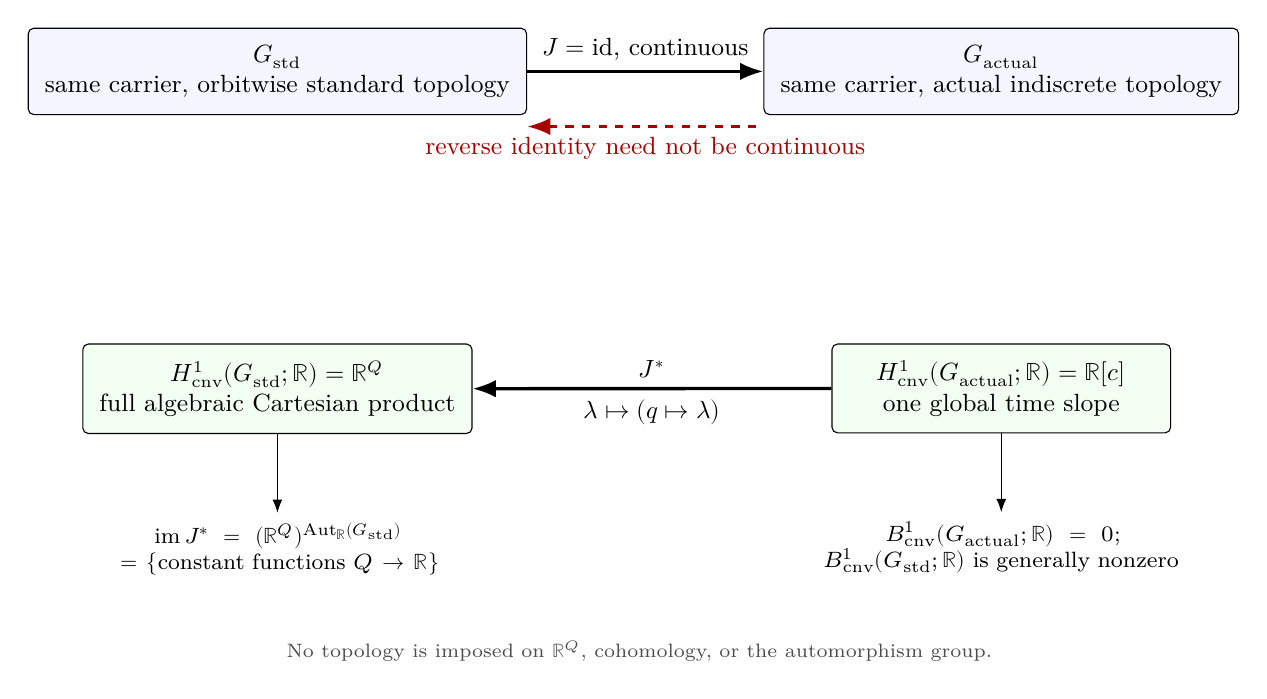
\begin{tikzpicture}[
  >=Latex,
  every node/.style={font=\small,align=center},
  box/.style={draw,rounded corners=2pt,fill=blue!4,inner sep=6pt,minimum width=43mm},
  cbox/.style={draw,rounded corners=2pt,fill=green!5,inner sep=6pt,minimum width=43mm},
  stop/.style={draw=red!65!black,very thick,dashed},
  note/.style={font=\footnotesize,align=center,text width=46mm}
]
  \node[box] (std) {$\Gstd$\\same carrier, orbitwise standard topology};
  \node[box,right=30mm of std] (act) {$\Gactual$\\same carrier, actual indiscrete topology};
  \draw[->,very thick] (std) -- node[above] {$J=\mathrm{id}$, continuous} (act);
  \draw[<-,stop] ([yshift=-7mm]std.east) -- node[below,text=red!65!black] {reverse identity need not be continuous} ([yshift=-7mm]act.west);

  \node[cbox,below=29mm of std] (hstd) {$H^1_{\cnv}(\Gstd;\R)=\R^Q$\\full algebraic Cartesian product};
  \node[cbox,below=29mm of act] (hact) {$H^1_{\cnv}(\Gactual;\R)=\R[c]$\\one global time slope};
  \draw[<-,very thick] (hstd) -- node[above] {$J^*$} node[below] {$\lambda\mapsto(q\mapsto\lambda)$} (hact);

  \node[note,below=10mm of hstd] (diag) {$\operatorname{im}J^*=(\R^Q)^{\operatorname{Aut}_{\R}(\Gstd)}$\\$=\{\text{constant functions }Q\to\R\}$};
  \node[note,below=10mm of hact] (bdry) {$B^1_{\cnv}(\Gactual;\R)=0$;\\$B^1_{\cnv}(\Gstd;\R)$ is generally nonzero};
  \draw[->,thin] (hstd) -- (diag);
  \draw[->,thin] (hact) -- (bdry);

  \node[font=\scriptsize,text=black!70,below=6mm of $(diag.south)!0.5!(bdry.south)$]
    {No topology is imposed on $\R^Q$, cohomology, or the automorphism group.};
\end{tikzpicture}
}
\caption{Same carrier, one-sided topology, and contravariant cohomology.
The actual line enters the standardized full product as the strict invariant
constant diagonal.  Standardized boundaries can be nonzero even though
actual boundaries vanish.}
\label{fig:same-carrier-diagonal}
\end{figure}

In prose, the upper row of \cref{fig:same-carrier-diagonal} says that the
identity $J$ is continuous from the finer orbitwise standard topology to the
actual indiscrete topology, while the reverse identity is not continuous.
The lower row reverses direction because cohomology is contravariant:
$J^*$ sends the single actual slope to the same slope on every orbit.  The
image is exactly the constant diagonal fixed by strict automorphisms.  The
display also records two nontransfer statements: actual coboundaries vanish,
standardized coboundaries generally do not, and the product $\R^Q$ is purely
algebraic.

\FloatBarrier

\subsection{Fixed-prime four-way application}
\label{sec:four-way}

Fix a rational prime $p$.  The source and actual-topology premises already
used in \cref{cor:packet-period} put the whole packet in the common-lattice
category with $H=(\log p)\Z$.  The packet need not be transitive; indeed the
standardization is designed for an arbitrary nonempty bare orbit set.

\begin{corollary}[Fixed-prime comparison]
\label{cor:packet-comparison}
Let $Q_p$ denote only the underlying set of fixed-prime packet orbits.  Put
the standard $\R/(\log p)\Z$ topology on every orbit of the same packet set
and take their coproduct.  Then
\begin{gather}
\label{eq:packet-comparison}
 \Gamma_p^{\mathrm{std}}\rtimes\R
 \xrightarrow{\ J_p\ }
 \Gamma_p^{\mathrm{actual}}\rtimes\R,\\
 \Hcnv^1(\Gamma_p^{\mathrm{actual}}\rtimes\R;\R)=\R[c],
 \qquad
 \Hcnv^1(\Gamma_p^{\mathrm{std}}\rtimes\R;\R)=\R^{Q_p},\notag\\
 \rho_p(\im J_p^*)
 =\{\text{constant functions on }Q_p\}
 =(\R^{Q_p})^{\AutR(\Gamma_p^{\mathrm{std}}\rtimes\R)},\notag
\end{gather}
and there is a canonical abstract-group extension
\begin{equation}
\label{eq:packet-automorphisms}
 1\longrightarrow
 \bigl(\R/(\log p)\Z\bigr)^{Q_p}
 \longrightarrow\AutR(\Gamma_p^{\mathrm{std}})
 \longrightarrow\Sym(Q_p)\longrightarrow1.
\end{equation}
Surjectivity and a noncanonical split use ZFC choice exactly as in
\cref{thm:automorphism-extension}.
\end{corollary}

\begin{proof}
Deninger's every-unit stabilizer and logarithmic clock supply the common
lattice; the actual-topology premise supplies the globally indiscrete
carrier.  Substituting $H=(\log p)\Z$ into
\cref{thm:std-topology,thm:equivalence,thm:automorphism-extension,thm:standard-h1,thm:invariant-diagonal}
gives each statement.
\end{proof}

The four records remain those of \cref{tab:packet-types}.  The actual
quotient $\Qactual$ is indiscrete, whereas $\Qdisc$ is discrete because the
inverse image of any subset is a union of open standardized components.
Only their bare underlying set is shared.  Nothing here provides its
cardinality, enumeration, measure, local triviality, arithmetic weighting,
or a topology inherited from the source.  Nor does the theorem compare
different primes or extend to an unregistered full suspension.

\begin{figure}[t]
\centering
\resizebox{\textwidth}{!}{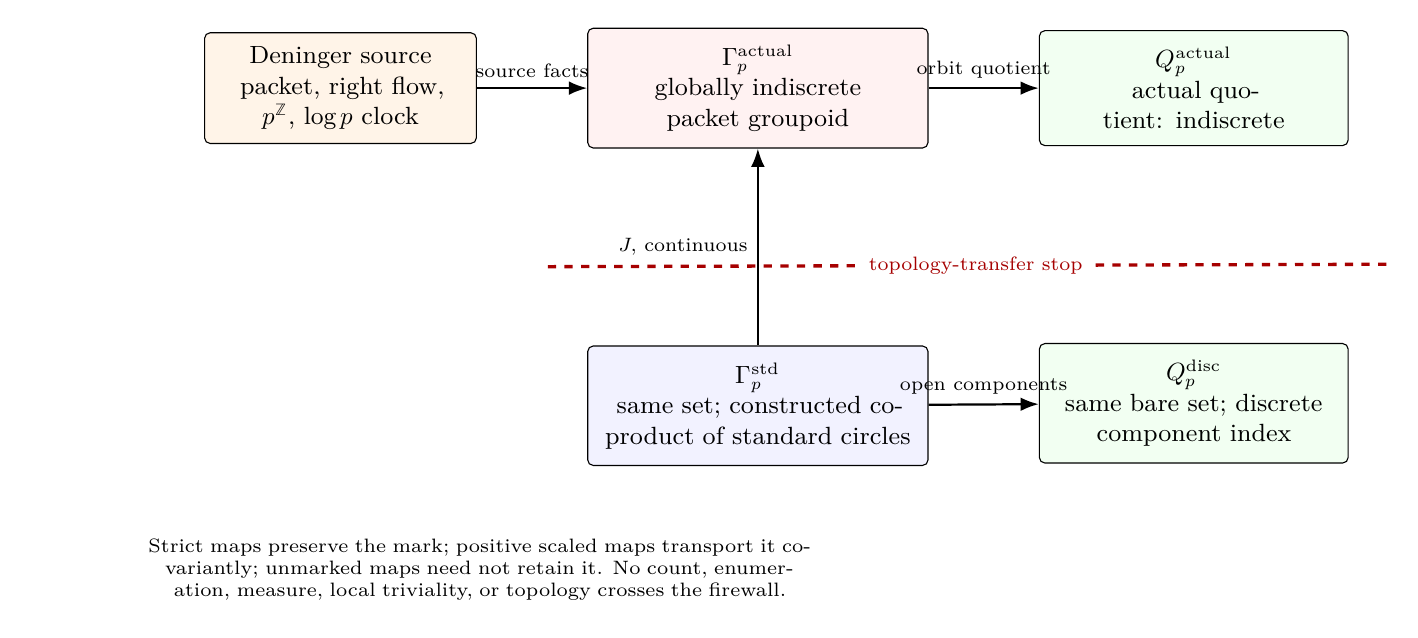
\begin{tikzpicture}[
  >=Latex,
  every node/.style={font=\small,align=center},
  src/.style={draw,rounded corners=2pt,fill=orange!9,inner sep=5pt,text width=31mm},
  act/.style={draw,rounded corners=2pt,fill=red!5,inner sep=6pt,text width=39mm},
  std/.style={draw,rounded corners=2pt,fill=blue!5,inner sep=6pt,text width=39mm},
  quot/.style={draw,rounded corners=2pt,fill=green!5,inner sep=6pt,text width=35mm},
  stop/.style={draw=red!65!black,very thick,dashed}
]
  \node[src] (den) {Deninger source\\packet, right flow, $p^{\Z}$, $\log p$ clock};
  \node[act,right=14mm of den] (ga) {$\Gamma_p^{\mathrm{actual}}$\\globally indiscrete packet groupoid};
  \node[quot,right=14mm of ga] (qa) {$Q_p^{\mathrm{actual}}$\\actual quotient: indiscrete};
  \draw[->,thick] (den) -- node[above,font=\scriptsize] {source facts} (ga);
  \draw[->,thick] (ga) -- node[above,font=\scriptsize] {orbit quotient} (qa);

  \node[std,below=25mm of ga] (gs) {$\Gamma_p^{\mathrm{std}}$\\same set; constructed coproduct of standard circles};
  \node[quot,below=25mm of qa] (qd) {$Q_p^{\mathrm{disc}}$\\same bare set; discrete component index};
  \draw[->,thick] (gs) -- node[above,font=\scriptsize] {open components} (qd);
  \draw[->,thick] (gs) -- node[left,font=\scriptsize] {$J$, continuous} (ga);

  \draw[stop] ([xshift=-5mm,yshift=10mm]gs.north west) -- ([xshift=5mm,yshift=10mm]qd.north east);
  \node[fill=white,text=red!65!black,font=\scriptsize] at ($(gs.north)!0.5!(qd.north)+(0,10mm)$)
    {topology-transfer stop};

  \node[font=\scriptsize,text width=112mm,below=8mm of gs.south east,anchor=north east]
    {Strict maps preserve the mark; positive scaled maps transport it covariantly; unmarked maps need not retain it. No count, enumeration, measure, local triviality, or topology crosses the firewall.};
\end{tikzpicture}
}
\caption{Fixed-prime owner and topology firewall.  Deninger supplies the
packet, right flow, every-unit $p^{\Z}$, and logarithmic clock; the companion
supplies the actual globally indiscrete packet topology; Paper~12 constructs
the same-set standardization and its discrete component index.  The stop bar
forbids topology transfer between the two quotient records.}
\label{fig:packet-four-way-firewall}
\end{figure}

In prose, \cref{fig:packet-four-way-firewall} follows the source facts into
the actual packet groupoid, then separates the actual quotient from the
constructed component index.  The downward arrow is the same-set topology
construction, not inheritance and not reflection.  At the categorical
boundary, strict maps retain the mark exactly, positive scaled maps obey
\cref{eq:scaled-covariance}, and unmarked isomorphisms can relate unequal
periods.  None of these statements enriches the bare orbit set arithmetically.

\FloatBarrier

\section{Deterministic controls, Route boundary, and limitations}
\label{sec:controls-route}

\subsection{Control receipt}

The frozen deterministic package passed 122/122 tests and produced 11 CSV
files with 3,486 rows.  It detected 14/14 intentional negatives.  The large
orbitwise-standardization ledger has 3,252 rows: 3,151 of them enumerate all
automorphisms of the selected finite cyclic models, while the other blocks
check topology, basepoint independence, coboundary/potential reconstruction,
the diagonal, invariants, and two v4 negative directions.  The other ledgers
check finite nerve identities, the $T_0$ boundary, continuous-additive
profiles, period formulas, category directions, packet-wide equality,
labels, and one-sided quotient topology.

\begin{table}[ht]
\centering
\small
\begin{tabularx}{\textwidth}{P{38mm}P{19mm}Y}
\toprule
Frozen control group & Rows & Exact manuscript role \\
\midrule
Orbitwise standardization $H^1$ & 3,252 & Finite topology,
automorphism, potential, diagonal, invariant, and wrong-direction witnesses. \\
Actual degree one and nerve/factorization & 143 & Finite face, $d^2$,
$T_0$/non-$T_0$, Cauchy-profile, and boundary witnesses. \\
Periods, packets, morphisms, labels, quotients & 70 & Exact finite examples
of period, every-unit, strict/scaled/unmarked, selectivity, and topology stops. \\
Target summary and explicit negatives & 21 & Nine target-level summaries
and twelve legacy negative-ledger rows. \\
\midrule
Total & 3,486 & 122/122 tests; 14/14 intentional negatives. \\
\bottomrule
\end{tabularx}
\caption{Frozen deterministic receipt.  Row groups are a presentation of
the manifest's 11 CSV files.  They are regression witnesses and falsifiers,
not proofs of universal, infinite-set, choice, topology, source, or
arithmetic statements.}
\label{tab:controls}
\end{table}

The generator and tests use the Python standard library only.  There is no
network call, external dataset, randomness, timestamp, fitting, hidden
target, zeta-zero table, trace, determinant, earlier-paper coefficient, or
analytic completion.  Exact arithmetic is used except for the frozen
$10^{-12}$ absolute tolerance on four displayed logarithm/square-root
values.  Checked-in, fresh-one, and fresh-two outputs were byte-identical in
the independently reviewed top-level run.  A duplicate-run orchestration
incident was discarded and contributed neither accepted evidence nor
residue; the top-level reproduction must not be run concurrently.  These
finite controls cannot prove the real or arbitrary-$Q$ theorems and do not
replace source verification.

\subsection{Typed Route result}

Eight owners were adjudicated separately.  \cref{tab:route} reports the
complete A0--A4 tuples but omits serialization fields and hashes, which
remain in the reproducibility ledger.  ``Exploratory'' is a scoped negative
prior, not weak positive evidence for a determinant, explicit formula, or
operator program.

\begin{table}[!htbp]
\centering
\scriptsize
\begin{tabularx}{\textwidth}{P{43mm}P{69mm}Y}
\toprule
Owner & Exact A0--A4 tuple & Verdict \\
\midrule
\texttt{GEN-INDISC-R-ACTION-CNV} & \TupleRejected & Rejected \\
\texttt{DEN-EF-ACTUAL-ORBIT-CNV-P-A} &
\TupleActual & Exploratory \\
\texttt{DEN-EF-ACTUAL-PACKET-CNV-P} &
\TupleActual & Exploratory \\
\texttt{DEN-EF-ACTUAL-ORBIT-MARKED-PERIOD-P-A} &
\TupleActual & Exploratory \\
\texttt{DEN-EF-ACTUAL-PACKET-MARKED-PERIOD-P} &
\TupleActual & Exploratory \\
\texttt{DEN-EF-STANDARD-PERIOD-QUOTIENT-P} &
\TupleStandard & Exploratory \\
\texttt{DEN-EF-STANDARDIZED-PACKET-H1-DIAGONAL-P} &
\TupleStandard & Exploratory \\
\texttt{UNMARKED-PERIOD-SCALING-CONTROL} &
\TupleUnmarked & Rejected \\
\bottomrule
\end{tabularx}
\caption{Exact eight-owner Route-A coordinate tuples: six exploratory and
two rejected.  Every A2--A4 coordinate fails; no coordinate may be spliced
across owners.}
\label{tab:route}
\end{table}

\FloatBarrier

Each owner explicitly uses
\texttt{NONE\_BY\_DESIGN\_NO\_DETERMINANT\_OBJECT}.  All nine required A2
metrics are negative or not applicable, every A3 and A4 coordinate fails,
every adversarial verdict is \texttt{STOP\_SCOPED}, and every Route-B flag is
false.  There are six Route-A exploratory records, two rejected records,
zero positive A2--A4 coordinates, and no Route-B file.  \RouteB{} remains
closed.  The generic and unmarked controls cannot donate evidence to the
source owners, and the constructed standard proxy cannot inherit the actual
topology or arithmetic selectivity.

\subsection{Limitations and prohibited inferences}
\label{sec:limitations}

The topology uniqueness and equivalence require a common nonzero cocompact
lattice $H=L\Z$.  Mixed stabilizers are outside that category.  The actual
all-degree factorization accepts arbitrary $T_0$ coefficients, but the
degree-one classification by slopes uses real coefficients and the direct
continuous Cauchy argument.  The standardized computation is degree one
only.  It does not calculate higher standardized cohomology.

The orbit set $Q$, and specifically $Q_p$, is bare.  We impose no
cardinality, enumeration, measure, local triviality, arithmetic weight, or
actual quotient topology.  The symbol $\R^Q$ means every algebraic function
$Q\to\R$; it does not mean $C(Q,\R)$, a direct sum, bounded functions, or a
topological product.  The automorphism extension is an extension of
abstract groups.  Its kernel map is canonical, its surjectivity uses ZFC
choice, and a split is noncanonical.

The invariant theorem is restricted to strict time-preserving equivariant
automorphisms.  It does not include positive scaled, unmarked,
orientation-reversing, or arbitrary abstract automorphisms.  The standard
topology is constructed from the action and mark.  It is not inherited from
the actual packet and is not a separated reflection.  The only continuous
same-set direction is standard to actual.

The fixed-prime corollary recovers a source-normalized mark already present
as the logarithm of Deninger's every-unit $p^{\Z}$.  It does not select primes,
compare primes, prove an orbit count, or extend to a full suspension.
Neither the theorem nor its controls define a trace, dynamical determinant,
analytic divisor, analytic continuation, quantization, completion, or
natural operator lift.  No such object may be inferred from the word
``cohomology,'' and \RouteB{} supplies no rescue.

The bounded literature statement remains exactly
\texttt{SUPPORTED\_WITHIN\_SEARCH through 2026-08-15}.  We make no claim of
being first, unprecedented, or globally without precedent.

The independently reviewed mathematical disposition is
\texttt{STANDALONE\_PASS}: the comparison in \cref{thm:main} closes the
earlier routine-reduction objection.  This is a claim-level disposition, not
a journal acceptance, citation, manuscript-quality, or public-release
authorization.  Public release remains conditional on the human and
companion-identity requirements stated below.

\section{Conclusion and successor boundary}
\label{sec:conclusion}

One carrier can support two sharply different continuous cohomology records.
With the actual global indiscrete topology, every continuous real
degree-one cocycle is one global time slope and every coboundary vanishes.
With the section-free coproduct of standard common-period orbits, independent
orbit slopes survive, producing the full algebraic product $\R^Q$, while
nonzero coboundaries also appear.  The continuous identity functor points
from standard to actual, so pullback embeds the actual line as the constant
diagonal.  The canonical automorphism extension shows that this diagonal is
exactly the strict invariant subspace.

For the fixed-prime packet, the same theorem recovers the source-normalized
$(\log p)\Z$ mark at every unit and keeps the actual packet, standardized
packet, actual quotient, and discrete component index separate.  The result
stops there.  A later Paper~13 may ask whether an independently defined
analytic object retains marked period information, but the present work
assumes no twist, completion, trace, determinant, operator, or spectral
construction for that successor.

\section*{Declarations}
\addcontentsline{toc}{section}{Declarations}

\paragraph{Author metadata and contributions.}
The provisional record is Liang Wang, Huazhong University of Science and
Technology, \href{mailto:wangliang.f@gmail.com}{wangliang.f@gmail.com}.
Final author list, academic unit, institution spelling, postal address if
required, corresponding-author status, email, ORCID, and all CRediT roles:
\textbf{AUTHOR TO CONFIRM}.  Repository history is not used to infer sole
authorship or contribution roles.

\paragraph{Funding.}
\textbf{AUTHOR TO CONFIRM}.  No absence of funding is inferred from the
current project record.

\paragraph{Competing interests.}
\textbf{AUTHOR TO CONFIRM}.  No absence of conflicts is inferred from
silence.

\paragraph{Acknowledgments.}
\textbf{AUTHOR TO CONFIRM}.

\paragraph{Ethics.}
This work consists of mathematical proof and deterministic controls.  No
human participant, animal, clinical intervention, personal, confidential,
or sensitive data enters the control manifest.  Venue-specific wording and
the final not-applicable declaration: \textbf{AUTHOR TO CONFIRM}.

\paragraph{Data and code availability.}
The local project contains the deterministic Python code, a manifest, and
11 generated CSV files.  It uses no external experimental dataset.  The
controls are regression witnesses and falsifiers, not proofs.  Public
repository, immutable tag or archive, license, and DOI:
\textbf{AUTHOR TO CONFIRM}.

\paragraph{AI assistance.}
AI assistance was used for research-protocol structuring, bounded source
discovery, exact-byte comparison, symbolic proof and deterministic-control
drafting, adversarial review, Route-record checking, and composition
planning.  The human author verified the cited sources and remains
responsible for every definition, theorem, computation, disclosure, and
publication claim.  The selected venue's current AI policy and final wording
must be confirmed before submission.

\paragraph{Companion and release status.}
The three companion records are unpublished and have no frozen immutable
public URL.  Before standalone public release, each load-bearing companion
dependency must either be bound to an honest immutable public record for the
audited version or be supplied self-containedly as an explicit premise or
proof.  Final venue, release date, public tag/archive, license, DOI, and
release authorization are \textbf{AUTHOR TO CONFIRM}.  Retained research
source PDFs are internal verification material and are excluded from every
public payload; the generated manuscript PDF is a project output, not a
source PDF.

\bibliographystyle{plainnat}
\begingroup
\raggedright
\bibliography{references}
\endgroup

\end{document}
